\documentclass{lug}

\usepackage{etoolbox}
\usepackage{etoolbox}
\usepackage{textcomp}
\usepackage[nodisplayskipstretch]{setspace}
\usepackage{xspace}
\usepackage{enumitem}
\usepackage{array}

\setminted{autogobble,breaklines,mathescape,fontsize=\tiny}

\newcolumntype{C}{>{\centering\arraybackslash}p{0.3\textwidth}}
\newcolumntype{D}{>{\centering\arraybackslash}p{0.6\textwidth}}

\makeatletter
\newlength\beamerleftmargin
\setlength\beamerleftmargin{\Gm@lmargin}
\makeatother

\setitemize{label=\usebeamerfont*{itemize item}%
  \usebeamercolor[fg]{itemize item}
  \usebeamertemplate{itemize item}}

\AtBeginSection[]{
  \begin{frame}
     \vfill
     \centering
     \includegraphics[width=2cm]{\secimage}

     \vspace{1cm}

     \begin{beamercolorbox}[sep=10pt,center]{title}
        \usebeamerfont{title}\insertsectionhead\par%
     \end{beamercolorbox}
     \vfill 
  \end{frame}
}

\makeatletter
\patchcmd{\beamer@sectionintoc}{\vskip1.5em}{\vskip0.5em}{}{}
\makeatother

\newcommand{\pmidg}[1]{\parbox{\widthof{#1}}{#1}}
\newcommand{\splitslide}[4]{%
    \noindent
    \begin{minipage}{#1 \textwidth - #2 }
        #3
    \end{minipage}%
    \hspace{ \dimexpr #2 * 2 \relax }%
    \begin{minipage}{\textwidth - #1 \textwidth - #2 }
        #4
    \end{minipage}
}
\setbeamerfont{footnote}{size=\tiny}

\title{Web Assembly}
\author{Sam Sartor}
\institute{Mines Linux Users Group}

\begin{document}

\newcommand{\secimage}{graphics/html_icon}
\section{Client Code}

\begin{frame}{Introduction}

\end{frame}

\renewcommand{\secimage}{graphics/sad_js}
\section{JavaScript}

\begin{frame}{On a dark and stormy night \dots}
    \begin{center}

        \textbf{The year is 1995.} Netscape Communications Corporation is
        dying. In a frantic attempt to one-up Microsoft, the company decides to
        embed a scripting language into the Netscape browser.
        
        \vspace{2ex}
        
        They give \textbf{Brendan Eich} 10 days to make a prototype.

        \vspace{2ex}

        Eich dreams of Scheme. He wants his new language to be elegant, fast,
        and pure. \textbf{But it is too late.} The lawyers at Netscape have made a deal
        with Sun Microsystems.

        \vspace{2ex}
        
        It will be known as \textbf{JavaScript}.
    \end{center}
\end{frame}

\begin{frame}{The Result}
    \begin{center}
        \includegraphics[width=\textwidth]{graphics/js_the_good}
    \end{center}
\end{frame}

\begin{frame}{This page uses 800 thousand lines of JavaScript}
    \vspace*{-4pt}%
    \hspace*{-\beamerleftmargin}%
    \includegraphics[width=\paperwidth]{graphics/pivotal_tracker}
\end{frame}

\renewcommand{\secimage}{graphics/emscripten_icon}
\section{Emscripten}

\begin{frame}{We need C}
    \splitslide{0.75}{1em}{\begin{itemize}
        \item People start writing games in JavaScript
        \item Why can't we use the Unity game engine?
        \item It's written in C
        \item Browsers don't run C
        \item Browsers only run JavaScript
        \item What if we compiled C to JavaScript?
    \end{itemize}}{\pmidg{
        \includegraphics[width=\columnwidth]{graphics/html5_logo} \\
        \vspace{1cm} \\
        \includegraphics[width=\columnwidth]{graphics/unity_logo}
    }}
\end{frame}

\begin{frame}{Emscripten}
    \begin{center}
        Introducing\dots\\
        \includegraphics[height=2cm]{graphics/emscripten_logo} \\
        \vspace{1cm}
        \textit{It compiles things to JavaScript!}
    \end{center}
\end{frame}

\begin{frame}{asm.js Example}
    \begin{center}\begin{tabular}{CD}
        C & asm.js \\
        \inputminted{c}{code/factorial.c} &
        \inputminted{js}{code/factorial.asm.js}
    \end{tabular}\end{center}
\end{frame}

\begin{frame}{That was a Bad Idea}
    \splitslide{0.75}{1em}{
        JavaScript was designed for\dots

        \vspace{1ex}

        \begin{tabular}{c l}
            {\color{green}\checkmark} & Crazy people \\
            {\color{yellow}$\bullet$} & Humans \\
            {\color{red}$\times$} & Computers
        \end{tabular}

        \vspace{3ex}

        Why compile low-level $\to$ high-level?

        \vspace{3ex}

        Why don't we have \emph{machine code for the web?}

    }{\pmidg{
        \includegraphics[width=\columnwidth]{graphics/machine_code}
    }}
\end{frame}

\renewcommand{\secimage}{graphics/wasm_logo}
\section{Web Asssembly}

\begin{frame}{Which Direction?}
    \begin{center}
        {
            \Huge
            \pmidg{\includegraphics[height=2cm]{graphics/js_logo}}
            {\color{red}$\nleftarrow$} 
            \pmidg{\includegraphics[height=2cm]{graphics/c_logo}}
            {\color{green}$\rightarrow$}
            \pmidg{\includegraphics[height=2cm]{graphics/wasm_logo}}
        }

        \vspace{2cm}

        \pmidg{\includegraphics[height=4ex]{graphics/emscripten_logo}}
        can compile your code to \textit{Web Assembly}!
    \end{center}
\end{frame}

\begin{frame}{WASM Example}
    \begin{center}\begin{tabular}{CCC}
        C & WASM Text & WASM Binary \\
        \inputminted{c}{code/factorial.c} &
        \inputminted{asm}{code/factorial.wasm.txt} &
        \inputminted{text}{code/factorial.wasm.hex}
    \end{tabular}\end{center}
\end{frame}

\begin{frame}{Software in the Browser}
    \pmidg{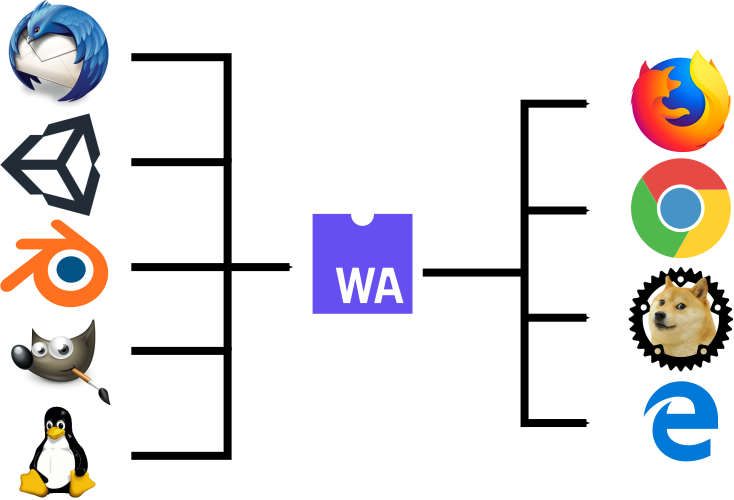
\includegraphics[width=\columnwidth]{graphics/wasm_chain}}
\end{frame}

\renewcommand{\secimage}{graphics/javascript_disabled}
\section{Practical WASM}

\renewcommand{\secimage}{graphics/c_logo}
\section{C/C++}

\renewcommand{\secimage}{graphics/rust_logo}
\section{Rust}

\renewcommand{\secimage}{graphics/stdweb_logo}
\section{stdweb}

\end{document}
